\documentclass[12pt]{article}
\usepackage[english]{babel}
\usepackage[utf8x]{inputenc}
\usepackage{amsmath}
\usepackage{graphicx}
\usepackage{subcaption}
\usepackage[export]{adjustbox}
\PassOptionsToPackage{hyphens}{url}
\usepackage{hyperref}

\graphicspath{ {../../Images/} }

\usepackage{xcolor}

\definecolor{codegreen}{rgb}{0,0.6,0}
\definecolor{codegray}{rgb}{0.5,0.5,0.5}
\definecolor{codepurple}{rgb}{0.58,0,0.82}
\definecolor{backcolour}{rgb}{0.95,0.95,0.92}

\hypersetup{
    colorlinks=true,
    linkcolor=blue,
    filecolor=magenta,      
    urlcolor=blue,
}
\usepackage{listings}
\lstdefinestyle{mystyle}{
    backgroundcolor=\color{backcolour},   
    commentstyle=\color{codegreen},
    keywordstyle=\color{magenta},
    numberstyle=\tiny\color{codegray},
    stringstyle=\color{codepurple},
    basicstyle=\ttfamily\footnotesize,
    breakatwhitespace=false,         
    breaklines=true,                 
    captionpos=b,                    
    keepspaces=true,                 
    numbers=left,                    
    numbersep=5pt,                  
    showspaces=false,                
    showstringspaces=false,
    showtabs=false,                  
    tabsize=2
}
\lstset{style=mystyle}

\begin{document}

\begin{titlepage}

\newcommand{\HRule}{\rule{\linewidth}{0.5mm}} 

\center
-------------------------------------------------------------------------------------

\textsc{\LARGE Politenico di Milano}\\[1cm]
\textsc{\Large Dipartimento Elettronica, Informazione e Bioingegneria}\\[0.5cm] 
\textsc{\large Final IoT Project}\\[0.5cm] 

%----------------------------------------------------------------------------------------
%	TITLE SECTION
%----------------------------------------------------------------------------------------

\HRule \\[0.4cm]
{ \huge \bfseries Keep Your Distance}\\[0.4cm]
\HRule \\[1.5cm]
 
%----------------------------------------------------------------------------------------
%	AUTHOR SECTION
%----------------------------------------------------------------------------------------

\begin{minipage}{0.4\textwidth}
	\begin{flushleft} \large
		\emph{Author:}\\
		Francesco \textsc{Monti}\\
		Matr: 919755 
	\end{flushleft}
\end{minipage}
~
\begin{minipage}{0.4\textwidth}
	\begin{flushright} \large
		\emph{Supervisor:} \\
		Dr. Edoardo \textsc{Longo}\\
		Dr. Matteo \textsc{Cesana}
	\end{flushright}
\end{minipage}\\[1.5cm]


%----------------------------------------------------------------------------------------
%	DATE SECTION
%----------------------------------------------------------------------------------------

{\large \today}\\[2cm] 

%----------------------------------------------------------------------------------------
%	LOGO SECTION
%----------------------------------------------------------------------------------------

\begin{figure}[h]
	\begin{subfigure}{0.5\textwidth}
		
\includegraphics[width=150pt, left]{Logo_Politecnico_Milano.png}
	\end{subfigure} 
	\begin{subfigure}{0.5\textwidth}
		
\includegraphics[width=100pt, right]{Ant_Lab_Logo.png}
	\end{subfigure}
\end{figure} 
 
%----------------------------------------------------------------------------------------

\vfill

\end{titlepage}
\begin{abstract}
This document contains the documentation for the final project of the course ``Internet of Things'', Academic Year 2019/2020. \\
This document has been also uploaded on the following GitHub repository: \url{https://github.com/Framonti/IoT_Projects}\\
\end{abstract}
\subsection{TinyOS App}
The logic of the TinyOS app is indeed very simple: it opens the radio and pings its presence (broadcasting its Mote ID) every half second. If it receives a message, it internally saves the ID of the sender by logging it and then it sends an alarm through the collaboration of Cooja, Node-RED and ITTT. 

In order to saves the messages, we declared a part of the flash memory of the device as reserved for logging. It would be possible to easily extend our application to read the logs (e.g. after a timeout, or if the memory is full), preprocess them (e.g. counting how many times the same device was logged) and finally send the data to a gateway. We remember that local preprocessing in IoT is usually recommended for reducing the size of messages.
\subsection{Simulation}
\begin{figure}[h]
	\begin{subfigure}{0.32\textwidth}
		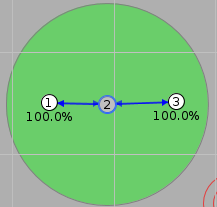
\includegraphics[width=100pt, left]{linear-topology.png}
	\end{subfigure} 
	\begin{subfigure}{0.32\textwidth}
		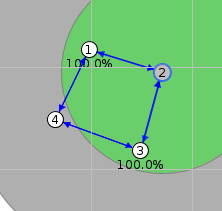
\includegraphics[width=100pt, center]{ring-topology.png}
	\end{subfigure}
	\begin{subfigure}{0.32\textwidth}
		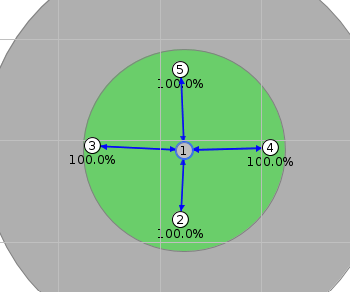
\includegraphics[width=100pt, right]{star-topology.png}
	\end{subfigure}
	\caption{Topology examples: From left to right, linear, ring, star topology}
	\label{fig:topologies}
\end{figure} 
We simulate our application using both TOSSIM and Cooja. We tried six different topologies using up to six motes (e.g. \ref{fig:topologies}). The simulation results and the topologies can be found in the folder \textit{``Sim\_Results''}. We point out a couple of important details:
\begin{itemize}
\item We can build the app for both telosb and micaz devices (\textit{make telosb} and \textit{make micaz}), but TOSSIM doesn't work with the Loggers nor the printf, because it's not able to simulate the flash memory nor the printf function. In order to obtain the simulations, we commented away the related code. A dbg statement replace the printf functionality, so it's still possible to see and validate the message exchanges. 
\item Another problem arose while simulating (\textit{python2 RunSimulationScript.py}), probably due to the small RAM available to the VM. We had to simulate the topologies one by one (by modifying line 52 of the Python script).
\item We split the simulations in different files, depending on the topology used. A \textit{``readme.txt''} file in the \textit{``Topologies Used''} folder describes the topologies.
\item The Cooja simulation contains only the printf statements; due to some compatibility issues the messages contains some strange characters, which we removed in Node-RED before firing ITTT requests. 
\end{itemize}

\subsection{Node-RED and ITTT}
\begin{figure}[h]
	\centering
	\captionsetup{justification=centering}
	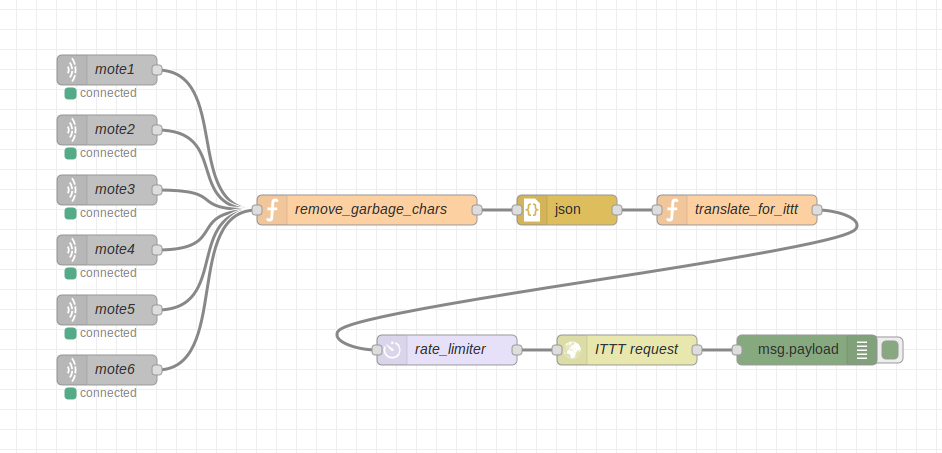
\includegraphics[width=\textwidth]{red-node-final.png}	
	\caption{Node-RED Design}
	\label{fig:red-node}
\end{figure}
We finally connects the messages sent by the motes to Node-RED through Cooja. Figure \ref{fig:red-node} shows the design. We can see that each mote is connected thanks to a TCP socket, then all the messages are preprocessed, transformed into a JSON object and sent to ITTT using a HTTP POST request. 

In ITTT we defined a simple rule, that fires an e-mail in order to simulate the alarm of a possible real application (\ref{fig:ittt-event}). 

\begin{figure}[h]
	\centering
	\captionsetup{justification=centering}
	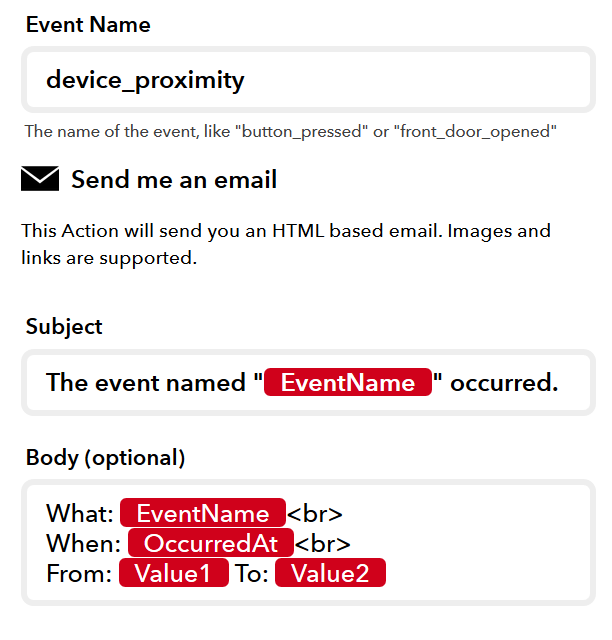
\includegraphics[width=200pt]{ittt-event.png}	
	\caption{ITTT Event}
	\label{fig:ittt-event}
\end{figure}

By simulating our application in Cooja, we received some e-mails (e.g. \ref{fig:mail}). We can see that ITTT has created an e-mail for the event ``device\_proximity'', including the Timestamp of the interaction, the Sender and the Receiver (identified with their Mote ID).


\begin{figure}[h]
	\centering
	\captionsetup{justification=centering}
	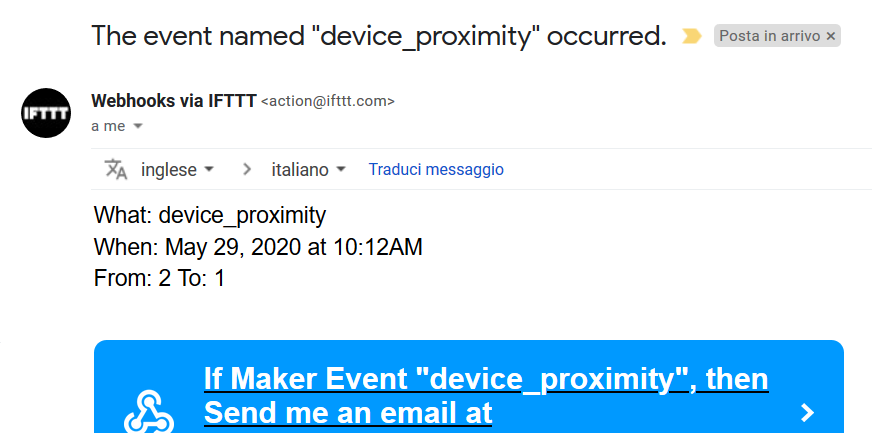
\includegraphics[width=200pt]{mail.png}	
	\caption{Mail Received by ITTT}
	\label{fig:mail}
\end{figure}



\end{document}